\documentclass[12pt]{article}

\usepackage[margin=2cm]{geometry}
\usepackage{amsmath}
\usepackage{multicol}
\usepackage{nopageno}
\usepackage{SIunits}
\usepackage{graphicx}
\usepackage{enumerate}
\usepackage{enumitem}
%\usepackage{mathabx}
\usepackage{wasysym}


% for making bond drawings
\usepackage{chemfig}
% Global bond settings
\setchemfig{
  atom sep=18pt,               % fixed bond length
  double bond sep=2pt,       % spacing between the two bars
  bond style={line width=0.8pt}
}


% for centering figures on page while in an enumerated/itemized list:
\usepackage{changepage} % in the preamble
\makeatletter
\newenvironment{centerinpage}
  {%
    \par\noindent
    \hspace*{-\@totalleftmargin}% back to page margin (covers all nested list indents)
    \begin{minipage}{\textwidth}% fixed to page width (ignores widened \linewidth)
      \centering
  }
  {%
    \end{minipage}\par
  }
\makeatother

%%%%%%%%%%%%%%%%%%%%%%%%%%%%%%%%%%%%%%%%%%%%%%%%%%%%%
% For putting links in the document (both to sections and hyperlinks)
\usepackage{hyperref}
\usepackage{url}
\hypersetup{
    colorlinks=true,     % false: boxed links; true: colored links
    linkcolor=red,       % color of internal links
    citecolor=blue,      % color of links to bibliography
    filecolor=blue,      % color of file links
    urlcolor=blue        % color of external links
}
% below, use \url{http://www.nytimes.com} (they will be urlcolor)
%%%%%%%%%%%%%%%%%%%%%%%%%%%%%%%%%%%%%%%%%%%%%%%%%%%%%


%%%%%%%%%%%%%%%%%%%%%%%%%%%%%%%%%%%%%%%%%%%%%%%%%%%%%
% for the events page boxes

% boxed regions
\usepackage{tcolorbox}
\tcbuselibrary{skins,breakable}

% fonts & spacing
\usepackage{lmodern}
\usepackage{microtype}
\usepackage{calc}


% small helper macros (adjust these)
\newcommand{\boxheight}{4.2cm}   % height for each event box
\newcommand{\boxfont}{\scriptsize} % change to \tiny or \footnotesize as desired
\newcommand{\linelen}{0.95\linewidth} % timeline line length

%%%%%%%%%%%%%%%%%%%%%%%%%%%%%%%%%%%%%%%%%%%%%%%%%%%%%
\newcommand{\rmd}{\ensuremath{{\rm d}}}
%\newcommand{\vv}[1]{\ensuremath{\vec{#1}}}
\newcommand{\vv}[1]{\ensuremath{\mathbf{#1}}}
\newcommand{\ee}[1]{\ensuremath{\mathbf{e}_{#1}}}
%%%%%%%%%%%%%%%%%%%%%%%%%%%%%%%%%%%%%%%%%%%%%%%%%%%%%



\begin{document}

\begin{center}
{\Large Evaporation and the radiative-convective equilibrium}
\end{center}
%%%%%%%%%%%%%%%%%%%%%%%%%%%%%%%%%%%%%%%%%%%%%%%%
%%%%%%%%%%%%%      overview         %%%%%%%%%%%%%%%%%%%%%
%%%%%%%%%%%%%%%%%%%%%%%%%%%%%%%%%%%%%%%%%%%%%%%%

\noindent In lab this week we examine the {\bf psychrometric chart} (relating relative humidity to absolute humidity) and the {\bf phase diagram} for water (depicting the coexistence curve between liquid water and water vapor near 0$\degree$C --- both are reproduced here on a later page.  The phase diagram is useful for understanding the evaporation of water exposed to air, because in that case the relevant pressure is not the atmospheric pressure, $p_\text{atm}$, but instead the {\bf partial pressure}, $e$, defined as
	%
	\begin{equation*}
	e = f  \times p_\text{atm} = \left( \frac{n_{\text{H}_2 \text{O}}}{n_{\text{H}_2 \text{O}} + n_\text{dry air}} \right) \times p_\text{atm}\,,
	\end{equation*}
	%
where you can see that partial pressure is found by multiplying the atmospheric pressure by $f$, the {\bf mole fraction of water in air}.  In lab you re-write this mole fraction in terms of the {\bf absolute humidity}, AH.  That new expression is:
	%
	\begin{equation*}
	\begin{split}
	e &= \left( \frac{ 
	\frac{m_{\text{H}_2 \text{O}}}{m_\text{dry air}}  \cdot  \frac{M_\text{dry air}}{M_{\text{H}_2 \text{O}}} 
	}
	{ \frac{m_{\text{H}_2 \text{O}}}{m_\text{dry air}}  \cdot \frac{M_\text{dry air}}{M_{\text{H}_2 \text{O}}}  + 1 } \right) \times p_\text{atm} \\
	& \\
	& =  
	\left(
	\frac{ \text{AH} \cdot 1.6}{ \text{AH} \cdot 1.6 + 1} 
	\right) \times p_\text{atm}
	\end{split}
	\end{equation*}
	%
where the mass ratio  $\frac{m_{\text{H}_2 \text{O}}}{m_\text{dry air}}$  is the absolute humidity read from the vertical axis of the psychrometric chart (but expressed as a pure ratio, e.g., $\unit{7}{\gram} / \unit{1}{\kilo\gram} = \unit{7}{\gram} / \unit{1000}{\gram} = 0.007$), and where the ratio of the molar masses is $M_\text{dry air} / M_{\text{H}_2 \text{O}}  =  28.8/18 = 1.6$.  So now you can:
	%
	\begin{itemize}
	\item Look up or measure the ``weather conditions'': relative humidity (\%) and ambient temperature.
	\item Use the psychrometric chart to convert these to an absolute humidity value, AH.
	\item Calculate the associated partial pressure of water in air, using the final equation above.
	\item Determine the vaporization temperature (liquid to vapor) from the phase diagram.
	\end{itemize}
	%
This vaporization temperature --- which is called ``the boiling point'' in a {\em pure} water liquid-vapor transition --- is called the {\bf dew point}. 


\newpage
%%%%%%%%%%%%%%%%%%%%%%%%%%%%%%%%%%%%%%%%%%%%%%%%
%%%%%%%%%%%%%      questions         %%%%%%%%%%%%%%%%%%%%%
%%%%%%%%%%%%%%%%%%%%%%%%%%%%%%%%%%%%%%%%%%%%%%%%

\begin{enumerate}

\item {\bf The dew point and water evaporation} Let's calculate the dew point temperature for a few different locations with diverse weather conditions.  In each case, draw a horizontal line on the phase diagram provided corresponding to your calculated partial pressure (label the line its location/conditions). Draw a dot on the line where it crosses the coexistence curve and a star on the line at the associated ambient temperature value.
	%
	\begin{enumerate}
	\item Let's start with ``indoor conditions.'' Modern air conditioning and heating is designed not only to keep the temperature at ``room temperature'' (look this up in $\degree$C), but also a comfortable 50\% relative humidity.  
	\item Now let's do Allendate/Grand Rapids yesterday in the afternoon. You can google for ``\verb|NWS 7 day grand rapids|'' and then navigate to the ``3 day History'' link (remember to convert temperatures from Fahrenheit to Celsius\ldots google can do this for you). Do you remember, was it comfortable outside (both in terms of temperature and humidity)?  
	\item On the search box of the NWS page, navigate to a different city where you expect that conditions were less humid than here.  Again look up their afternoon data.
	\item Repeat the previous but for a location where you expect the conditions were more humid than here.
	\end{enumerate}

\item {\bf Why dew?}  Using our understanding of evaporation developed in the previous question and in lab, let's try to answer some qualitative questions about our surroundings.
	%
	\begin{enumerate}
	\item In lab this week we do an experiment where the temperature of a beaker of water is slowly lowered by the introduction of ice.  What did you observe (or would you expect to observe) on the outside of the beaker and when? 
	\item Look up the temperature of a standard refrigerator.  If you remove a jar of olives from the fridge, 
	\end{enumerate}


\item {\bf Radiative-Convective Equilibrium Temperature} In prior weeks we made estimates of the Earth's equilibrium temperature.  In fact this is the driving question of the first half of the course: What do we expect to be the temperature of the Earth?  Let's review our prior results and then push forward to a new (and basically final) answer using the mechanism of energy transfer by evaporation.
	%
	\begin{enumerate}
	\item st
	\end{enumerate}


\end{enumerate}
\newpage
%%%%%%%%%%%%%%%%%%%%%%%%%%%%%%%%%%%%%%%%%%%%%%%%%%%%
%%%%%%%%%%               phase diagram and psychrometric chart              %%%%%%%%%%%%%
%%%%%%%%%%%%%%%%%%%%%%%%%%%%%%%%%%%%%%%%%%%%%%%%%%%%


\begin{figure}
\centering
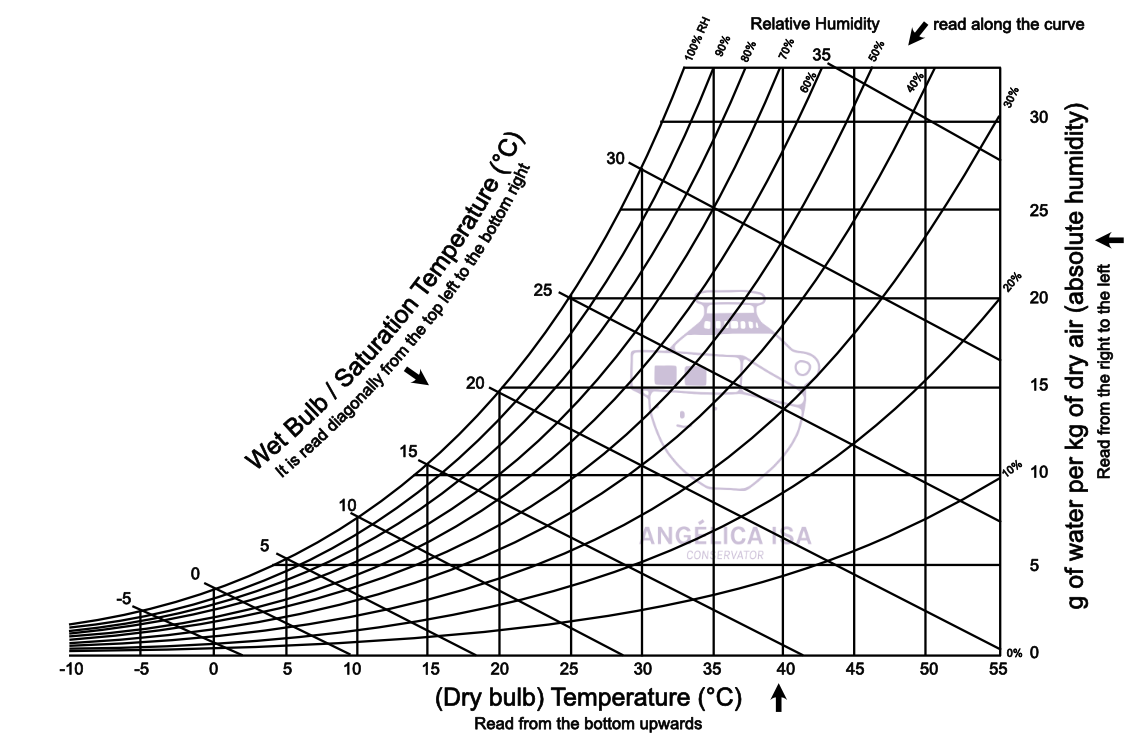
\includegraphics[width=0.95 \textwidth]{images/08_psychrometric_angelica-isa.png}\\
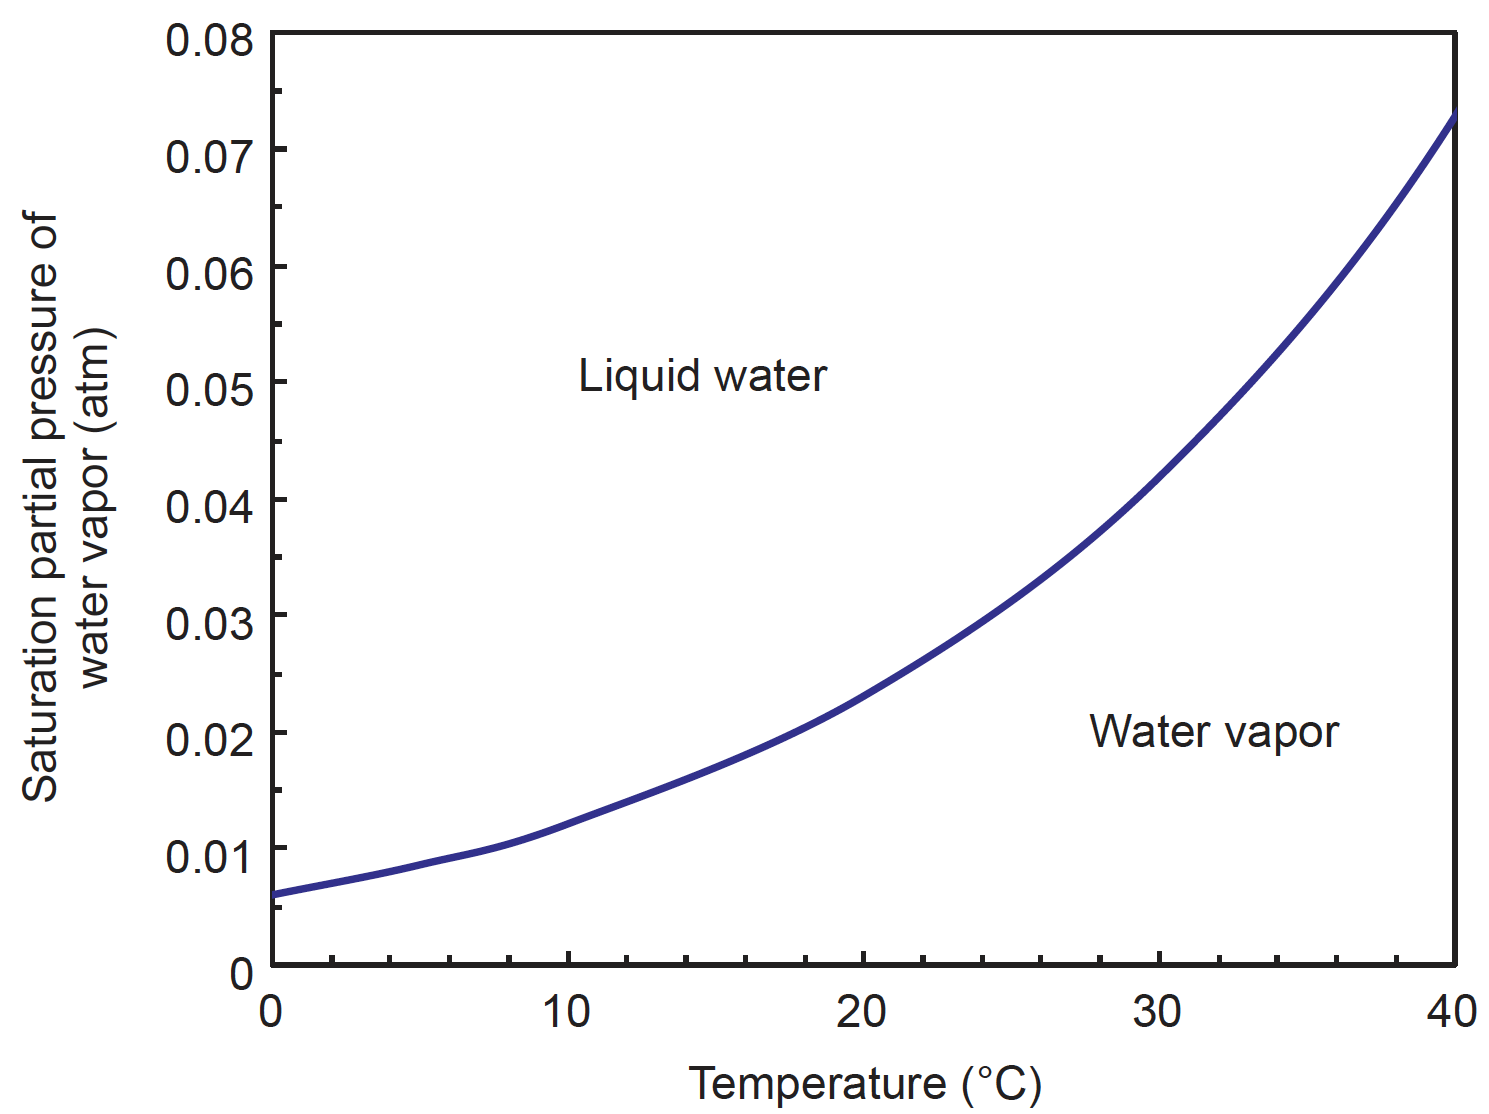
\includegraphics[width=0.95 \textwidth]{images/08_pressure-vs-temperature-clausius-clapeyron_mathez-fig-1-2_no-caption.png}
\caption{ \label{fig:08_psychrometric-and-phase-diagrams}
{\bf Top}: Psychrometric chart for water at standard pressure conditions $\unit{1}{atm} = \unit{101}{\kilo\pascal}$ (from angelicaisa.com). {\bf Bottom}: Phase transition coexistence curve for water near the triple point (from Mathez \& Smerdon).
}
\end{figure}




%%%%%%%%%%%%%%%%%%%%%%%%%%%%%%%%%%%%%%%%%%%%%%%%%%%%
%%%%%%%%%%                                  References                                %%%%%%%%%%%%%%%%
%%%%%%%%%%%%%%%%%%%%%%%%%%%%%%%%%%%%%%%%%%%%%%%%%%%%
%\noindent {\bf Data Sources}: 



\end{document}
